\documentclass[12pt, letterpaper]{article}
\usepackage[T1]{fontenc}
\usepackage[utf8]{inputenc}
\usepackage[spanish]{babel}
\usepackage{hyperref}
\usepackage{graphicx}
\usepackage{xcolor}
\usepackage{titlesec}
\usepackage{fancyhdr}
\usepackage[margin=2cm, top=2cm,includefoot]{geometry}
\usepackage[outputdir=pdf]{minted}
\usemintedstyle{emacs}
\setminted[sql]{
  frame=lines,
  framesep=2mm,
  baselinestretch=1.2,
  fontsize=\footnotesize,
  breaklines,
}

%  not bold
\titleformat{\subsubsection}
  {\normalfont\fontfamily{phv}\fontsize{11}{15}\selectfont}{\thesubsubsection}{1em}{}

\begin{document}
    \begin{titlepage}
        \centering
        {\bfseries\LARGE Ejercicios SQL}\par
        {}
    \end{titlepage}

    \tableofcontents

    \newpage

    \section{Tienda Informática}
    \subsection{Modelo entidad relación}
    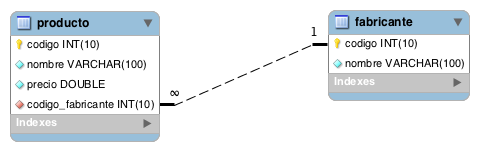
\includegraphics[width=0.8\textwidth,height=0.8\textheight,keepaspectratio]{assets/entidad-relacion.png}

    \subsection{Crear base de datos}
   \begin{minted}[linenos]{sql}
  DROP DATABASE IF EXISTS tienda;
   CREATE DATABASE tienda CHARACTER SET utf8mb4;
   USE tienda;
   
   CREATE TABLE fabricante (
     id INT UNSIGNED AUTO_INCREMENT PRIMARY KEY,
     nombre VARCHAR(100) NOT NULL
   );
   
   CREATE TABLE producto (
     id INT UNSIGNED AUTO_INCREMENT PRIMARY KEY,
     nombre VARCHAR(100) NOT NULL,
     precio DOUBLE NOT NULL,
     id_fabricante INT UNSIGNED NOT NULL,
     FOREIGN KEY (id_fabricante) REFERENCES fabricante(id)
   );
   
   INSERT INTO fabricante VALUES(1, 'Asus');
   INSERT INTO fabricante VALUES(2, 'Lenovo');
   INSERT INTO fabricante VALUES(3, 'Hewlett-Packard');
   INSERT INTO fabricante VALUES(4, 'Samsung');
   INSERT INTO fabricante VALUES(5, 'Seagate');
   INSERT INTO fabricante VALUES(6, 'Crucial');
   INSERT INTO fabricante VALUES(7, 'Gigabyte');
   INSERT INTO fabricante VALUES(8, 'Huawei');
   INSERT INTO fabricante VALUES(9, 'Xiaomi');
   
   INSERT INTO producto VALUES(1, 'Disco duro SATA3 1TB', 86.99, 5);
   INSERT INTO producto VALUES(2, 'Memoria RAM DDR4 8GB', 120, 6);
   INSERT INTO producto VALUES(3, 'Disco SSD 1 TB', 150.99, 4);
   INSERT INTO producto VALUES(4, 'GeForce GTX 1050Ti', 185, 7);
   INSERT INTO producto VALUES(5, 'GeForce GTX 1080 Xtreme', 755, 6);
   INSERT INTO producto VALUES(6, 'Monitor 24 LED Full HD', 202, 1);
   INSERT INTO producto VALUES(7, 'Monitor 27 LED Full HD', 245.99, 1);
  
   INSERT INTO producto VALUES(10, 'Impresora HP Deskjet 3720', 59.99, 3);
   INSERT INTO producto VALUES(11, 'Impresora HP Laserjet Pro M26nw', 180, 3);
   \end{minted}
  

  \subsection{Consultas sobre una tabla}
  \subsubsection{Lista el nombre de todos los productos que hay en la tabla \textit{\textbf{producto}}}
  \mint{sql}|SELECT nombre  FROM producto;|

  \subsubsection{Lista los \textit{\textbf{nombres}} y los \textit{\textbf{precios}} de todos los \textit{\textbf{productos}} de la tabla \textit{\textbf{producto}} }
  \mint{sql}|SELECT nombre, precio  FROM producto;|

  \subsubsection{Lista todas las columnas de la tabla \textit{\textbf{producto}}}
  \mint{sql}|SELECT * FROM producto;|

  \subsubsection{Lista el \textit{\textbf{nombre}} de los productos y el \textit{\textbf{precio en euros}} y el \textit{\textbf{precio en dólares estadounidenses}}}
  \mint{sql}|SELECT nombre, precio / 21, precio / 18 FROM producto;|

  \subsubsection{Lista el \textit{\textbf{nombre}} de los productos, el \textit{\textbf{precio en euros}} y el \textit{\textbf{precio en dólares}}. Utiliza los siguientes alias para las columnas: \textit{\textbf{nombre de producto, euros, dólares}}}
  \mint{sql}|SELECT nombre AS "nombre de producto", precio / 18 AS euro, precio / 21 AS dólares FROM producto;|

  \subsubsection{Lista los \textit{\textbf{nombres}} y los \textit{\textbf{precios}} de todos los productos de la tabla \textit{\textbf{producto}}, convirtiendo los \textit{\textbf{nombres}} a \textit{\textbf{mayúsculas}}}
  \mint{sql}|SELECT UPPER(nombre) AS "NOMBRE PRODUCTO", precio AS PRECIO FROM producto;|
  
  \subsubsection{Lista los \textit{\textbf{nombres}} y los \textit{\textbf{precios}} de todos los productos de la tabla \textit{\textbf{producto}}, convirtiendo los \textit{\textbf{nombres}} a \textit{\textbf{minúsculas}}}
  \mint{sql}|SELECT LOWER(nombre), precio FROM producto;|

  \subsubsection{Lista el \textit{\textbf{nombre}} de todos los fabricantes en una columna, en otra columna obtenga en \textit{\textbf{mayúsculas los dos primeros caracteres del nombre del fabricante}}}
   \mint{sql}|SELECT nombre, UPPER(LEFT(nombre, 2)) AS caracters FROM fabricante;|

  \subsubsection{Lista los \textit{\textbf{nombres}} y los \textit{\textbf{precios}} de todos los productos de la tabla \textit{\textbf{producto}}, \textit{\textbf{redondeando}} el valor preciso}
   \mint{sql}|SELECT nombre, ROUND(precio) as precio FROM producto;|

  \subsubsection{Lis los \textit{\textbf{nombres}} y los \textit{\textbf{precios}} de todos los productos de la tabla \textit{\textbf{producto}}, \textit{\textbf{truncando}} el valor del \textit{\textbf{precio}} para mostrarlo \textit{\textbf{sin ninguna cifra decimal}}}
   \mint{sql}|SELECT nombre, TRUNCATE(precio, 0) as precio FROM producto;|

  \subsubsection{Lista el \textit{\textbf{indentificador}} de los fabricantes que tienen productos el tabla \textit{\textbf{producto}}}
   \mint{sql}|SELECT fabricante.id FROM fabricante LEFT JOIN producto ON fabricante.id = producto.id_fabricante|
  
  \subsubsection{Lista el \textit{\textbf{indetificador}} de los fabricantes que tienen productos en la tabla \textit{\textbf{producto}}, \textit{\textbf{eliminando}} los identificadores que aparecen repetidos - \textit{\textbf{PENDIENTE}} }
   \mint{sql}||

  \subsubsection{Lista los \textit{\textbf{nombres}} de los fabricantes \textit{\textbf{ordenados}} de forma \textit{\textbf{ascendente}}}
   \mint{sql}|SELECT nombre FROM fabricante ORDER BY nombre ASC;|

  \subsubsection{Lista los \textit{\textbf{nombres}} de los fabricantes \textit{\textbf{ordenados}} de forma \textit{\textbf{descendente}}}
   \mint{sql}|SELECT nombre FROM fabricante ORDER BY nombre DESC;|

  \subsubsection{Lista los nombres}
   \mint{sql}|select|
\end{document}